\chapter{Fundamentos de Elasticidade}\label{sec.fund_elast}

\section{Introdu\c{c}\~ao}
A teoria formal da propaga\c{c}\~ao de ondas s\'ismicas repousa nas intera\c{c}\~oes entre as part\'iculas infinitesimais discretas do meio \`a medida que uma deforma\c{c}\~ao se propaga. \'E muito dif\'icil estudar individualmente cada uma dessas intera\c{c}\~oes, mas dados experimentais que foram coletados como resultados dessas intera\c{c}\~oes sugerem que as mesmas podem ser consideradas em conjunto. Assim, o estudo da propaga\c{c}\~ao de ondas s\'ismicas atrav\'es de camadas de subsuperf\'icie num material discretizado pode ser feito considerando o meio como cont\'inuo, e tais estudos s\~ao os objetos da \textit{mec\^anica do cont\'inuo}. 

No desenvolvimento te\'orico da mec\^anica do cont\'inuo n\~ao s\~ao consideradas as caracter\'isticas at\^omicas da mat\'eria bem como as intera\c{c}\~oes entre essas part\'iculas, ou seja, a mat\'eria n\~ao \'e estudada do ponto de vista microsc\'opico. Segundo \cite{slawinski}, tal abordagem se justifica pelo fato de que a mat\'eria \'e formada por part\'iculas suficientemente pouco espa\c{c}adas e suas caracter\'isticas e comportamento podem ser descritos por fun\c{c}\~oes cont\'inuas e diferenci\'aveis. Assim, \'e assummido que elementos infinitesimais da mat\'eria t\^em as mesmas propriedades observadas em experimentos macrosc\'opicos, pois essa hip\'otese permite a cria\c{c}\~ao de um modelo matem\'atico abstrato \textit{efetivo} na descri\c{c}\~ao da realidade f\'isica. Como exemplo, vamos considerar a cor de um objeto. Pr\'otons e el\'etrons n\~ao possuem cor, mas os meios materiais (que s\~ao formados por pr\'otons e el\'etrons) t\^em a capacidade de absorver ou refletir determinados comprimentos de ondas eletromagn\'eticas as quais determinam a cor de cada meio. Outros conceitos da mec\^anica do cont\'inuo s\~ao elasticidade, viscosidade, fric\c{c}\~ao, rigidez, etc, como veremos mais a frente.


\section{Fatos experimentais}
A teoria sobre elasticidade est\'a baseada em conceitos primitivos e conclus\~oes estabelecidas a partir de fatos experimentais verificados em v\'arios textos sobre o assunto como \cite{liu}, \cite{dahlem} e \cite{slawinski}. Adicionalmente, em geral as equa\c{c}\~oes que governam a propaga\c{c}\~ao de ondas em meios el\'asticos s\~ao n\~ao-lineares. Contudo, em experimentos s\'ismicos foi constatado que aspectos importantes da propaga\c{c}\~ao de ondas podem ser analisados a partir de equa\c{c}\~oes lineares, resultando numa abordagem chamada \textit{teoria da elasticidade linearizada}.

\subsection{Deforma\c{c}\~ao}

A \textit{deforma\c{c}\~ao} de um meio el\'astico cont\'inuo \'e a mudan\c{c}a na posi\c{c}\~ao dos pontos que comp\~oem o corpo em rela\c{c}\~ao uns aos outros. Ou seja, h\'a uma mudan\c{c}a relativa entre os pontos e n\~ao um deslocamento do corpo como um todo e sem mudan\c{c}a de sua forma, caso em que ter\'iamos um \textit{movimento r\'igido}. Nesta subse\c{c}\~ao estamos interessados nas caracter\'isticas geom\'etricas relativas \`a deforma\c{c}\~ao de um corpo. N\~ao estamos considerando as causas de deforma\c{c}\~ao de um corpo, como aplica\c{c}\~ao de carga ou varia\c{c}\~ao de temperatura, nem discutiremos a composi\c{c}\~ao do material, assumindo apenas que o mesmo seja cont\'inuo e el\'astico. Assim, vamos relacionar as caracter\'isticas geom\'etricas de um corpo antes da deforma\c{c}\~ao com as caracter\'isticas ap\'os a deforma\c{c}\~ao.

\subsection{Dedu\c{c}\~ao do Tensor de Deforma\c{c}\~oes}\label{sec.deriva_deforma}

Para determinar o tensor de deforma\c{c}\~oes vamos considerar dois pontos pertencentes ao espaco $\mathbb{R}^3$ bastante pr\'oximos um do outro denotados por
\begin{align*}
\mathbf{x}&=(x_1,x_2,x_3)\quad\text{e}\\
\mathbf{y}=\mathbf{x}+d\mathbf{s}&=(x_1+dx_1,x_2+dx_2,x_3+dx_3),
\end{align*}
e que podem ser observados na figura \ref{fig.deformacao_meio}. O quadrado da dist\^ancia entre esses dois pontos \'e
\begin{equation}\label{eq.dist_antes_defor}
\norm{d\mathbf{s}}^2=(dx_1)^2+(dx_2)^2+(dx_3)^2.
\end{equation}
\begin{figure}
\centering
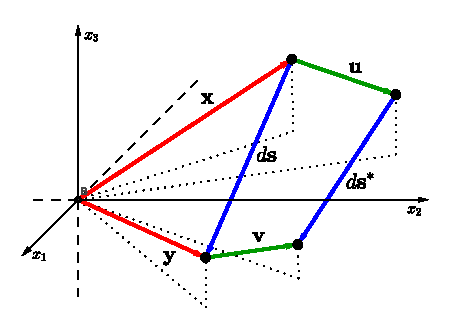
\includegraphics[scale=1.4]{deformacao_meio}
\caption{\textit{Mudan\c{c}a na posi\c{c}\~ao relativa entre os pontos que comp\~oem um  meio el\'astico cont\'inuo.}}
\label{fig.deformacao_meio}
\end{figure}
A aplica\c{c}\~ao de uma deforma\c{c}\~ao depende do ponto de aplica\c{c}\~ao, ou seja, a deforma\c{c}\~ao aplicada no ponto $\mathbf{x}$ difere da aplica\c{c}\~ao no ponto $\mathbf{y}$. Caso o vetor que d\'a a deforma\c{c}\~ao tenha componentes constantes, n\~ao teremos uma deforma\c{c}\~ao relativa, apenas uma transla\c{c}\~ao dos pontos. Assim, podemos definir o \textit{vetor de deslocamento} para cada ponto de aplica\c{c}\~ao
\begin{align*}
\mathbf{u}(\mathbf{x})&=(u_1,u_2,u_3),\\
\mathbf{v}(\mathbf{y})&=(v_1,v_2,v_3),
\end{align*}
e som\'a-los aos respectivos pontos $\mathbf{x}$ e $\mathbf{y}$ para obter suas posi\c{c}\~oes ap\'os a deforma\c{c}\~ao,
\begin{align*}
\mathbf{x}^*&=(x_1+u_1,x_2+u_2,x_3+u_3)\\
\mathbf{y}^*&=(x_1+dx_1+v_1,x_2+dx_2+v_2,x_3+dx_3+v_3).
\end{align*}
Subtraindo, obtemos o vetor que d\'a a diferen\c{c}a entre os pontos ap\'os a deforma\c{c}\~ao
\begin{equation}\label{eq.dist_apos_defor}
d\mathbf{s}^*=(dx_1+v_1-u_1,dx_2+v_2-u_2,dx_3+v_3-u_3).
\end{equation}
Como a varia\c{c}\~ao entre os pontos $\mathbf{x}$ e $\mathbf{y}$ \'e infinitesimal, vamos aplicar a expans\~ao de Taylor de segunda ordem em torno do ponto $\mathbf{x}$ e desprezar o resto de Lagrange para escrever as componentes de $\mathbf{v}$ em fun\c{c}\~ao das componentes de $\mathbf{u}$, aproximadamente,
\begin{align*}
v_1&\approx u_1+\frac{\partial u_1}{\partial x_1}\Bigg\vert_{\mathbf{x}}dx_1+\frac{\partial u_1}{\partial x_2}\Bigg\vert_{\mathbf{x}}dx_2+\frac{\partial u_1}{\partial x_3}\Bigg\vert_{\mathbf{x}}dx_3\\\\
v_2&\approx u_2+\frac{\partial u_2}{\partial x_1}\Bigg\vert_{\mathbf{x}}dx_1+\frac{\partial u_2}{\partial x_2}\Bigg\vert_{\mathbf{x}}dx_2+\frac{\partial u_2}{\partial x_3}\Bigg\vert_{\mathbf{x}}dx_3\\\\
v_3&\approx u_3+\frac{\partial u_3}{\partial x_1}\Bigg\vert_{\mathbf{x}}dx_1+\frac{\partial u_3}{\partial x_2}\Bigg\vert_{\mathbf{x}}dx_2+\frac{\partial u_3}{\partial x_3}\Bigg\vert_{\mathbf{x}}dx_3.
\end{align*}
Substituindo esses valores na equa\c{c}\~ao \ref{eq.dist_apos_defor}, simplificando e introduzindo a nota\c{c}\~ao de somat\'orio temos
\begin{equation*}
d\mathbf{s}^*\approx\left(dx_1+\sum_{i=1}^3\frac{\partial u_1}{\partial x_i}\Bigg\vert_{\mathbf{x}}dx_i\,,\,dx_2+\sum_{i=1}^3\frac{\partial u_2}{\partial x_i}\Bigg\vert_{\mathbf{x}}dx_i\,,\,dx_3+\sum_{i=1}^3\frac{\partial u_3}{\partial x_i}\Bigg\vert_{\mathbf{x}}dx_i\right).
\end{equation*}
O quadrado da dist\^ancia entre os pontos ap\'os a deforma\c{c}\~ao \'e dado por
\begin{equation*}
\norm{d\mathbf{s}^*}^2\approx\left(dx_1+\sum_{i=1}^3\frac{\partial u_1}{\partial x_i}\Bigg\vert_{\mathbf{x}}dx_i\right)^2+\left(dx_2+\sum_{i=1}^3\frac{\partial u_2}{\partial x_i}\Bigg\vert_{\mathbf{x}}dx_i\right)^2+\left(dx_3+\sum_{i=1}^3\frac{\partial u_3}{\partial x_i}\Bigg\vert_{\mathbf{x}}dx_i\right)^2.
\end{equation*}
Abrindo cada uma das parcelas quadr\'aticas, temos
\begin{align*}
\norm{d\mathbf{s}^*}^2&\approx(dx_1)^2+2\,dx_1\,\sum_{i=1}^3\frac{\partial u_1}{\partial x_i}\Bigg\vert_{\mathbf{x}}dx_i+\left(\sum_{i=1}^3\frac{\partial u_1}{\partial x_i}\Bigg\vert_{\mathbf{x}}dx_i\right)^2\\\\
&+(dx_2)^2+2\,dx_2\,\sum_{i=1}^3\frac{\partial u_2}{\partial x_i}\Bigg\vert_{\mathbf{x}}dx_i+\left(\sum_{i=1}^3\frac{\partial u_2}{\partial x_i}\Bigg\vert_{\mathbf{x}}dx_i\right)^2\\\\
&+(dx_3)^2+2\,dx_3\,\sum_{i=1}^3\frac{\partial u_3}{\partial x_i}\Bigg\vert_{\mathbf{x}}dx_i+\left(\sum_{i=1}^3\frac{\partial u_3}{\partial x_i}\Bigg\vert_{\mathbf{x}}dx_i\right)^2.
\end{align*}
Pela equa\c{c}\~ao \ref{eq.dist_antes_defor}, a coluna  da esquerda \'e $\norm{d\mathbf{s}}^2$. Como estamos trabalhando com quantidades infinitesimais, podemos negligenciar a coluna da direita por se tratar do quadrado do gradiente de cada componente do vetor de deslocamento num produto escalar com o vetor que d\'a a dist\^ancia entre os pontos $\mathbf{x}$  e $\mathbf{y}$. A coluna do meio se desdobra em dezoito parcelas que podem ser reagrupadas num somat\'orio duplo. Assim,
\begin{equation*}
\norm{d\mathbf{s}^*}^2\approx\norm{d\mathbf{s}}^2+\sum_{i=1}^3\sum_{j=1}^3\left(\frac{\partial u_i}{\partial x_j}\Bigg\vert_{\mathbf{x}}+\frac{\partial u_j}{\partial x_i}\Bigg\vert_{\mathbf{x}}\right)dx_i\,dx_j,
\end{equation*}
onde o termo entre par\^enteses \'e definido como o \textit{tensor de deforma\c{c}\~ao} na teoria da elasticidade,
\begin{equation*}
\varepsilon_{i,j}=\frac{1}{2}\left(\frac{\partial u_i}{\partial x_j}\Bigg\vert_{\mathbf{x}}+\frac{\partial u_j}{\partial x_i}\Bigg\vert_{\mathbf{x}}\right),\qquad\text{e}\qquad i,j\,\in\,\{1,2,3\}.
\end{equation*}
Considerando deslocamentos infinitesimais, os componentes desse tensor nos permitem descrever as deforma\c{c}\~oes associadas a esses deslocamentos entre os pontos iniciais. Analisando as entradas do tensor vemos que se o vetor de deslocamento \'e constante ent\~ao $\epsilon_{i,j}=0$ para todo o tensor, e n\~ao h\'a deforma\c{c}\~ao, apenas movimento r\'igido como descrito anteriormente. Como se trata de uma matriz sim\'etrica, no espa\c{c}o $\mathbb{R}^3$ temos apenas seis componentes independentes para o tensor.

\subsection{Interpreta\c{c}\~ao Geom\'etrica do Tensor de Deforma\c{c}\~ao}

Existem basicamente dois tipos de deforma\c{c}\~oes descritas pelo tensor, uma onde podemos ter mudan\c{c}a de comprimento em alguma dimens\~ao ocasionando mudan\c{c}a de volume, mas sem mudan\c{c}a na forma do corpo estudado. Outra com mudan\c{c}a na forma mas sem mudan\c{c}a de volume. Vamos analisar como cada entrada do tensor \'e respons\'avel por altera\c{c}\~oes geom\'etricas do meio.

\subsubsection{Altera\c{c}\~ao Relativa de Comprimento}\label{sec.alte_compri}

Considerando o caso unidimensional, vamos aplicar as deforma\c{c}\~oes $\mathbf{u}$ e $\mathbf{v}$ aos pontos $\mathbf{x}=(x_1,0,0)$ e $\mathbf{y}=(x_1+dx_1,0,0)$, respectivamente,
\begin{equation*}
\mathbf{x}^*=(x_1+u_1,u_2,u_3)\quad\text{e}\quad\mathbf{y}^*=(x_1+dx_1+v_1,v_2,v_3).
\end{equation*}
Calculando a dist\^ancia entre os pontos ap\'os a deforma\c{c}\~ao temos
\begin{equation*}
d\mathbf{s}^*=(dx_1+v_1-u_1,v_2-u_2,v_3-u_3).
\end{equation*}
Analogamente a subse\c{c}\~ao \ref{sec.deriva_deforma}, vamos usar a expans\~ao de Taylor e ignorar o resto de Lagrange para escrever a primeira componente de $\mathbf{v}$ em fun\c{c}\~ao da primeira componente de $\mathbf{u}$. 
\begin{equation*}
v_1(\mathbf{y})=u_1(\mathbf{x})+\frac{\partial u_1}{\partial x_1}\Bigg\vert_{\mathbf{x}}dx_1+\frac{1}{2}\frac{\partial^2 u_1}{\partial x_1^2}\Bigg\vert_{\mathbf{x}}(dx_1)^2+\cdots
\end{equation*}
Novamente, utilizando a aproxima\c{c}\~ao para os dois primeiros termos e substituindo a primeira componente do vetor $d\mathbf{s}^*$, temos
\begin{equation}
dx_1^*\approx dx_1+\frac{\partial u_1}{\partial x_1}\Bigg\vert_{\mathbf{x}}dx_1\approx \left(1+\frac{\partial u_1}{\partial x_1}\Bigg\vert_{\mathbf{x}}\right)\,dx_1. 
\end{equation}
Usando a nota\c{c}\~ao dos componentes do tensor de deforma\c{c}\~ao, temos
\begin{equation}\label{eq.defor_unidi}
dx_1^*\approx(1+\epsilon_{11})\,dx_1.
\end{equation} 
Assim, vemos que $\epsilon_{11}$ \'e uma contra\c{c}\~ao ou dilata\c{c}\~ao ao longo do eixo $x_1$ e, analogamente, podemos demonstrar que $\epsilon_{22}$ e $\epsilon_{33}$ determinam a distens\~ao ou contra\c{c}\~ao ao longo dos eixos $x_2$ e $x_3$, respectivamente.
Utilizando um abuso de nota\c{c}\~ao, podemos escrever a express\~ao \ref{eq.defor_unidi} como
\begin{equation*}
\frac{dx_1^*}{dx_1}\approx \frac{\partial x_1+\partial u_1}{\partial x_1},
\end{equation*}
e desse jeito podemos perceber que o fator $(1+\epsilon_{11})$ \'e uma mudan\c{c}a relativa (citada na subse\c{c}\~ao \ref{sec.deriva_deforma}) no comprimento ao longo do eixo $x_1$ devido a deforma\c{c}\~ao.

\subsubsection{Altera\c{c}\~ao Relativa de Volume}

Para estudar as altera\c{c}\~oes no volume de um s\'olido el\'astico vamos considerar uma caixa retangular (paralelep\'ipedo) com dimens\~oes $\Delta x_1, \Delta x_2\,\text{e}\,\Delta x_3$ nas dire\c{c}\~oes dos eixos coordenados.  Dessa forma, o volume do paralelep\'ipedo \'e dado por\begin{equation*}
V=\Delta x_1\,\Delta x_2\,\Delta x_3.
\end{equation*}
Conforme subse\c{c}\~ao \ref{sec.alte_compri}, aplicando a mudan\c{c}a relativa de comprimento a cada uma das tr\^es dimens\~oes, temos que ap\'os a deforma\c{c}\~ao, o volume do s\'olido \'e dado por
\begin{align}\nonumber
V^*&=(1+\epsilon_{11})\Delta x_1\,(1+\epsilon_{22})\Delta x_2\,(1+\epsilon_{33})\Delta x_3\\\label{eq.altera_volume}
&=(1+\epsilon_{11})\,(1+\epsilon_{22})\,(1+\epsilon_{33})\,V.
\end{align}
Como a deforma\c{c}\~ao aplicada tem tamanho infinitesimal, estamos supondo que as altera\c{c}\~oes relativas de comprimento n\~ao fujam significativamente das dire\c{c}\~oes can\^onicas dos eixos coordenados, assim h\'a altera\c{c}\~ao apenas no volume do s\'olido e n\~ao no seu formato. Ainda por conta do valores infinitesimais de $\epsilon_{ii}$, podemos negligenciar os termos n\~ao lineares resultantes da multiplica\c{c}\~ao na equa\c{c}\~ao \ref{eq.altera_volume} e aproximar o volume ap\'os a deforma\c{c}\~ao para
\begin{equation}\label{eq.altera_volume_2}
V^*\approx(1+\epsilon_{11}+\epsilon_{22}+\epsilon_{33})\,V.
\end{equation}
Observe que $\epsilon_{11}+\epsilon_{22}+\epsilon_{33}$ \'e o tra\c{c}o do tensor de deforma\c{c}\~ao, pode ser calculado atrav\'es do divergente do vetor de deslocamento e ser\'a denotado por $\varphi$ definindo a \textit{dilata\c{c}\~ao},
\begin{align*}
\varphi &=\epsilon_{11}+\epsilon_{22}+\epsilon_{33}\\
&=\frac{\partial u_1}{\partial x_1}+\frac{\partial u_2}{\partial x_2}+\frac{\partial u_3}{\partial x_3}\\
&=\left(\frac{\partial}{\partial x_1},\frac{\partial}{\partial x_2},\frac{\partial}{\partial x_3}\right)\cdot(u_1,u_2,u_3)\\
&=\nabla\cdot \mathbf{u}.
\end{align*}
Como o tra\c{c}o de uma matriz \'e um escalar e este n\~ao se altera quando \'e aplicada uma transforma\c{c}\~ao nos eixos coordenados, temos que a dilata\c{c}\~ao e a consequente altera\c{c}\~ao no volume de um s\'olido n\~ao depende do sistema de coordenadas escolhido. Manipulando a equa\c{c}\~ao \ref{eq.altera_volume_2} podemos constatar que a dilata\c{c}\~ao se trata de uma mudan\c{c}a relativa do volume
\begin{equation*}
\frac{V^*-V}{V}\approx\epsilon_{11}+\epsilon_{22}+\epsilon_{33}.
\end{equation*}

\subsubsection{Altera\c{c}\~ao Relativa na Forma}

O tensor de deforma\c{c}\~ao tamb\'em descreve uma mudan\c{c}a no formato do corpo, conforme podemos acompanhar pela figura \ref{fig.deforma_formato}, onde um ret\^angulo \'e transformado num paralelogramo. 
\begin{figure}
\centering
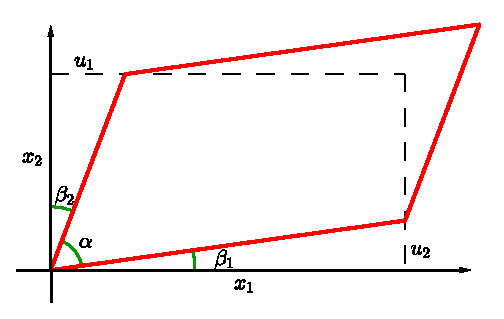
\includegraphics[scale=1.4]{deforma_formato}
\caption{\textit{Exemplo em duas dimens\~oes de como algumas componentes do tensor de deforma\c{c}\~ao promove a varia\c{c}\~ao no formato do meio.}}
\label{fig.deforma_formato}
\end{figure}
O angulo reto inicialmente formado pelos eixos coordenados $x_1$ e $x_2$ \'e reduzido a um \^angulo $\alpha$ que obedece \`a rela\c{c}\~ao
\begin{equation*}
\alpha=\frac{\pi}{2}-\beta_1-\beta_2,
\end{equation*}
onde $\beta_1$ e $\beta_2$ s\~ao os \^angulos formados pelos lados do paralelogramo e os eixos $x_1$ e $x_2$, respectivamente. Como a varia\c{c}\~ao angular \'e bastante pequena, temos que cada \^angulo $\beta_i$ pode ser aproximado por sua respectiva tangente, e considerando deslocamentos infinitesimais, temos
\begin{align*}
\beta_1+\beta_2&\approx\tan(\beta_1)+\tan(\beta_2)\\
&=\frac{\partial u_2}{\partial x_1}+\frac{\partial u_1}{\partial x_2}\\
&=2\epsilon_{12}=2\epsilon_{21}.
\end{align*}
Portanto, temos que o tensor de deforma\c{c}\~ao tamb\'em \'e respons\'avel pela altera\c{c}\~ao na dire\c{c}\~ao dos seguimentos que comp\~oem um corpo, mudando assim seu formato.


\subsection{Conserva\c{c}\~ao da Massa, Tens\~ao e o Equil\'ibrio do Momento Linear}\label{sec.massa_tensao_momen_lin}

O princ\'ipio de conserva\c{c}\~ao da massa \'e fundamental em mec\^anica do cont\'inuo na determina\c{c}\~ao da rela\c{c}\~ao entre o vetor de deslocamento $\mathbf{u}$ e a densidade de massa $\rho$ de um corpo. Por defini\c{c}\~ao, a quantidade de massa ocupando um volume $V$  num dado tempo $t$ \'e
\begin{equation*}
m=\iiint_V\rho\,dV,
\end{equation*}
onde tanto a massa como a densidade n\~ao dependem apenas do tempo mas tamb\'em da posi\c{c}\~ao $\mathbf{x}$. Fixado um volume $V$, a taxa de varia\c{c}\~ao da massa no tempo \'e dada por
\begin{equation}\label{eq.massa_1}
\frac{d}{dt}m=\iiint_V\frac{\partial\rho}{\partial t}dV.
\end{equation}
Assumindo que n\~ao h\'a destrui\c{c}\~ao nem produ\c{c}\~ao de massa dentro do volume, a varia\c{c}\~ao da massa se d\'a apenas pelo quantidade de massa que passa pelo volume, ou que passa atrav\'es de uma das superf\'icies que limita esse volume, o que pode ser escrito como
\begin{equation}\label{eq.massa_2}
\frac{dm}{dt}=-\iint_S\rho\,\mathbf{v}\cdot d\mathbf{S},
\end{equation}
onde $\mathbf{v}$ \'e a velocidade da quantidade de massa que atravessa a superf\'icie $S$. A superf\'icie infinitesimal $dS$ \'e pequena o suficiente para ser considerada plana e tem o mesmo fluxo de massa em todos os seus pontos, e o sinal negativo decorre do fato de que o vetor normal \`a superf\'icie aponta no sentido de sa\'ida do volume. 

Substituindo a equa\c{c}\~ao \ref{eq.massa_2} na equa\c{c}\~ao \ref{eq.massa_1} temos
\begin{equation}\label{eq.massa_3}
\iiint_V\frac{\partial\rho}{\partial t}dV=-\iint_S\rho\,\mathbf{v}\cdot d\mathbf{S},
\end{equation}
ou seja, a taxa de varia\c{c}\~ao da quantidade de massa num determinado volume \'e proporcional \`a taxa de varia\c{c}\~ao da quantidade de massa que atravessa a superf\'icie que limita esse volume. Pelo teorema do divergente temos que
\begin{equation}\label{eq.massa_divergente}
\iint_S\rho\,\mathbf{v}\cdot d\mathbf{S}=\iiint_V\nabla\cdot (\rho\,\mathbf{v})\,dV,
\end{equation}
onde substiutindo a equa\c{c}\~ao \ref{eq.massa_divergente} na equa\c{c}\~ao \ref{eq.massa_3} e agrupando os integrandos sob um mesmo volume, temos
\begin{equation*}
\iiint_V\left[\frac{\partial\rho}{\partial t}+\nabla\cdot (\rho\,\mathbf{v})\right]\,dV=0,
\end{equation*}
que \'e a equa\c{c}\~ao que descreve a \textit{conserva\c{c}\~ao de massa} num determinado volume $V$.

Em geral, as for\c{c}as agindo no interior de um meio continuo s\~ao as chamadas \textit{for\c{c}as de superf\'icie}, ou seja, quando um material \'e submetido ao contato de uma carga em sua superf\'ice, for\c{c}as internas se propagam no inteiror do material atrav\'es de outras superf\'icies internas e imagin\'arias provocando a deforma\c{c}\~ao desse material. Assim, podemos definir a \textit{tens\~ao} como o conjunto dessas for\c{c}as de superf\'ice, fazendo com que tens\~ao e deforma\c{c}\~ao estejam diretamente relacionadas. Matematicamente, tens\~ao m\'edia \'e definida como a for\c{c}a por unidade de \'area
\begin{equation}\label{eq.tensao_media}
\mathbf{\overline{T}}=\frac{\Delta\mathbf{F}}{\Delta S},
\end{equation}
e segundo o princ\'ipio fundamental da mec\^anica do cont\'inuo estabelecido por Cauchy, existe o limite para o valor da tens\~ao quando $\Delta S\to 0$,
\begin{equation*}
\mathbf{T}^{\mathbf{n}}=\lim_{\Delta S\to 0}\frac{\Delta\mathbf{F}}{\Delta S}=\frac{d\mathbf{F}}{dS}.
\end{equation*}
O vetor $\mathbf{n}$ \'e normal a superf\'icie de aplica\c{c}\~ao da tens\~ao $\mathbf{T}^{\mathbf{n}}$ e \'e \'util para identificar que determinada tens\~ao se aplica a determinada superf\'icie.

Al\'em das for\c{c}as de superf\'icie temos tamb\'em as for\c{c}as de corpo que agem \`a dist\^ancia como a for\c{c}a gravitacional ou a for\c{c}a el\'etrica que agem sobre um corpo material ou sobre uma carga el\'etrica, respectivamente. Denotando tal for\c{c}a por $\mathbf{f}(\mathbf{x},t)$ temos que a for\c{c}a total atuando num corpo \'e
\begin{equation}\label{eq.forca_total}
\mathbf{F}_T=\iint_S\mathbf{T}\,dS+\iiint_V\mathbf{f}\,dV,
\end{equation}
onde $V$ \'e o volume enclausurado pela superf\'icie $S$. Usando a defini\c{c}\~ao de for\c{c}a dada pela segunda lei de Newton, podemos reescrever a equa\c{c}\~ao \ref{eq.forca_total} como
\begin{equation}\label{eq.forca_total_2}
\frac{d}{dt}\iiint_V\rho\frac{d\mathbf{u}}{dt}\,dV=\iint_S\mathbf{T}\,dS+\iiint_V\mathbf{f}\,dV,
\end{equation}
onde $\mathbf{u}$ \'e o vetor deslocamento. A equa\c{c}\~ao \ref{eq.forca_total_2} estabelece o equil\'ibrio do \textit{momento linear}, ou seja, a taxa de varia\c{c}\~ao do momento linear de uma part\'icula no meio cont\'inuo \'e igual ao somat\'orio de for\c{c}as externas agindo nessa part\'icula. Discretizando a \'ultima integral da equa\c{c}\~ao acima podemos escrever
\begin{equation*}
\frac{1}{2}\sum_{i=1}^n\sum_{j=1}^n(\mathbf{F}_{ji}+\mathbf{F}_{ij}),
\end{equation*}
onde $\mathbf{F}_{ji}$ \'e a for\c{c}a exercida na part\'icula $i$ devida \`a part\'icula $j$. Pela terceira lei de Newton, for\c{c}as entre part\'iculas tem mesma intensidade e dire\c{c}\~ao e sentidos opostos, assim, $\mathbf{F}_{ji}=-\mathbf{F}_{ij}$. Mais ainda, uma part\'icula n\~ao exerce uma for\c{c}a em si mesma, ent\~ao $\mathbf{F}_{ii}=0$. Portanto, a equa\c{c}\~ao \ref{eq.forca_total_2} se resume a
\begin{equation*}
\frac{d}{dt}\iiint_V\rho\frac{d\mathbf{u}}{dt}\,dV=\iint_S\mathbf{T}\,dS.
\end{equation*}
Somente for\c{c}as externas s\~ao respons\'aveis por altera\c{c}\~oes no momento linear.

\subsection{O Tensor de Tens\~oes}\label{sec.tensor_tensoes}

Para deriva\c{c}\~ao do tensor de tens\~oes vamos utilizar o argumento do tetraedro de Cauchy, estudando as for\c{c}as agindo no inteiror de um meio cont\'inuo em rela\c{c}\~ao a um plano imagin\'ario com orienta\c{c}\~ao arbitr\'aria. O tetraedro \'e limitado pelos pontos $O(0,0,0)$, $X(x,0,0)$, $Y(0,y,0)$ e $Z(0,0,z)$, contendo faces ortogonais, $OYZ$, $XOZ$ e $XYO$ e a face obl\'iqua $XYZ$, conforme a figura \ref{fig.tetraedro}.
\begin{figure}
\centering
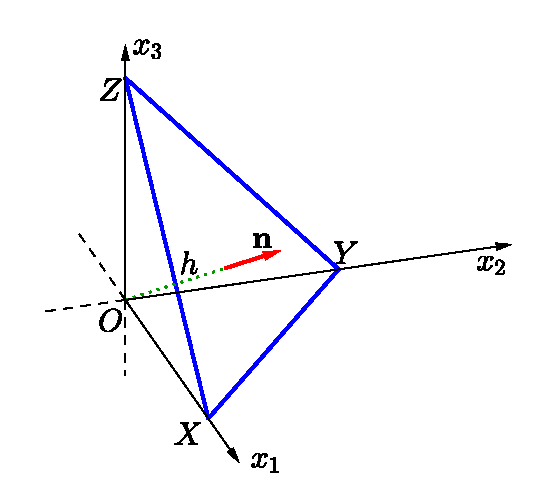
\includegraphics[scale=1]{tetraedro_cauchy}
\caption{\textit{Tetraedro de Cauchy, com for\c{c}as superficiais agindo em cada uma das faces ortogonais e na face obl\'iqua.}}
\label{fig.tetraedro}
\end{figure}

 Utilizando o equil\'ibro do momento linear dado pela equa\c{c}\~ao \ref{eq.forca_total_2}, podemos determinar a for\c{c}a agindo na face obl\'iqua de \'area $\Delta S$, considerando um tetraedro de dimens\~oes finitas.
\begin{equation}\label{eq.forca_total_3}
\overline{\rho}\,\Delta V\frac{d\overline{\mathbf{v}}}{dt}=\Delta \mathbf{F}+\Delta\mathbf{F}^{(\mathbf{e}_1)}+\Delta\mathbf{F}^{(\mathbf{e}_2)}+\Delta\mathbf{F}^{(\mathbf{e}_3)}+\overline{f}\Delta V,
\end{equation} 
onde $\Delta\mathbf{F}$ \'e a for\c{c}a superficial agindo na face obl\'iqua, $\Delta\mathbf{F}^{(\mathbf{e}_i)}$ \'e a for\c{c}a superficial agindo na face ortogonal cujo a normal \'e o eixo $x_i$, $\overline{f}$ \'e a for\c{c}a de campo agindo no tetraedro de volume $\Delta V$ e densidade $\rho$, e $\frac{d\overline{\mathbf{v}}}{dt}$ \'e a velocidade usada no c\'alculo da taxa de varia\c{c}\~ao do momento linear. As barras acima de cada s\'imbolo significam valores m\'edios para tetraedros de dimens\~oes finitas. Substituindo a equa\c{c}\~ao \ref{eq.tensao_media} na equa\c{c}\~ao \ref{eq.forca_total_3} temos
\begin{equation}\label{eq.forca_total_4}
\overline{\rho}\,\Delta V\frac{d\overline{\mathbf{v}}}{dt}=\mathbf{\overline{T}}^{(\mathbf{n})}\,\Delta S-\mathbf{\overline{T}}^{(\mathbf{e}_1)}\,\Delta S_1-\mathbf{\overline{T}}^{(\mathbf{e}_2)}\,\Delta S_2-\mathbf{\overline{T}}^{(\mathbf{e}_3)}\,\Delta S_3+\overline{f}\,\Delta V,
\end{equation}
onde $\Delta S_i$ \'e a \'area da face cujo a normal \'e o eixo $x_i$. Note, ainda pela figura \ref{fig.tetraedro}, que as faces ortogonais tem suas respectivas normais com a mesma dire\c{c}\~ao mas sentido oposto ao respectivo vetor unit\'ario $\mathbf{e}_i$ do eixo correspondente, da\'i o sinal negativo na equa\c{c}\~ao acima por conta da terceira lei de Newton. Para continuarmos nossa deriva\c{c}\~ao precisamos relacionar a \'area da face obl\'iqua com as \'areas das faces ortogonais. Observe que cada componente $n_i$ do vetor $\mathbf{n}$ \'e, por defini\c{c}\~ao,
\begin{align*}
n_1&=\mathbf{n}\cdot\mathbf{e}_1=\norm{\mathbf{n}}\,\norm{\mathbf{e}_1}\cos(X\hat{O}N)\\
n_2&=\mathbf{n}\cdot\mathbf{e}_2=\norm{\mathbf{n}}\,\norm{\mathbf{e}_2}\cos(Y\hat{O}N)\\
n_3&=\mathbf{n}\cdot\mathbf{e}_3=\norm{\mathbf{n}}\,\norm{\mathbf{e}_3}\cos(Z\hat{O}N)\\
\end{align*}
Usando a defini\c{c}\~ao de cosseno nos tri\^angulos $XON$, $YON$ e $ZON$ temos que
\begin{equation*}
h=\overline{XO}\,n_1=\overline{YO}\,n_2=\overline{ZO}\,n_3,
\end{equation*}
e calculando o volume do tetraedro em rela\c{c}\~ao a cada uma das faces temos
\begin{equation}\label{eq.volume_tetraedro}
\Delta V=\frac{1}{3}h\,\Delta S=\frac{1}{3}\overline{XO}\Delta S_1=\frac{1}{3}\overline{YO}\Delta S_2=\frac{1}{3}\overline{ZO}\Delta S_3,
\end{equation}
e da\'i temos a rela\c{c}\~ao entre as \'areas,
\begin{equation}\label{eq.relacao_areas}
\Delta S=\Delta S_in_i,\quad\text{onde}\quad i=1,2,3.
\end{equation}
Usando as equa\c{c}\~oes \ref{eq.volume_tetraedro} e \ref{eq.relacao_areas} podemos escrever a equa\c{c}\~ao \ref{eq.forca_total_4} como
\begin{equation*}
\overline{\rho}\,\frac{1}{3}h\,\Delta S\frac{d\overline{\mathbf{v}}}{dt}=\mathbf{\overline{T}}^{(\mathbf{n})}\,\Delta S-\mathbf{\overline{T}}^{(\mathbf{e}_1)}\,n_1\,\Delta S-\mathbf{\overline{T}}^{(\mathbf{e}_2)}\,n_2\,\Delta S-\mathbf{\overline{T}}^{(\mathbf{e}_3)}\,n_3\,\Delta S+\overline{f}\,\frac{1}{3}h\,\Delta S.
\end{equation*}
Cancelando $\Delta S$, temos
\begin{equation*}
\overline{\rho}\,\frac{1}{3}h\frac{d\overline{\mathbf{v}}}{dt}=\mathbf{\overline{T}}^{(\mathbf{n})}-\mathbf{\overline{T}}^{(\mathbf{e}_1)}\,n_1-\mathbf{\overline{T}}^{(\mathbf{e}_2)}\,n_2-\mathbf{\overline{T}}^{(\mathbf{e}_3)}\,n_3+\overline{f}\frac{1}{3}h.
\end{equation*}
Reduzindo o tetraedro de dimens\~oes finitas a um tetraedro infinitesimal, fazemos $h\to 0$ mantendo o v\'ertice $O$ centrado na origem e sem alterar a dire\c{c}\~ao de $h$,
\begin{equation*}
\mathbf{T}^{(\mathbf{n})}=\mathbf{T}^{(\mathbf{e}_1)}\,n_1+\mathbf{T}^{(\mathbf{e}_2)}\,n_2+\mathbf{T}^{(\mathbf{e}_3)}\,n_3.
\end{equation*}
Em termos matriciais, temos
\begin{align}\nonumber
\mathbf{T}^{(\mathbf{n})}&=
\begin{bmatrix}
T_1^{(\mathbf{e}_1)}\\
T_2^{(\mathbf{e}_1)}\\
T_3^{(\mathbf{e}_1)}
\end{bmatrix}
n_1+
\begin{bmatrix}
T_1^{(\mathbf{e}_2)}\\
T_2^{(\mathbf{e}_2)}\\
T_3^{(\mathbf{e}_2)}
\end{bmatrix}
n_2+
\begin{bmatrix}
T_1^{(\mathbf{e}_3)}\\
T_2^{(\mathbf{e}_3)}\\
T_3^{(\mathbf{e}_3)}
\end{bmatrix}
n_3\\\label{eq.matriz_tensao}
&=
\begin{bmatrix}
T_1^{(\mathbf{e}_1)}&T_1^{(\mathbf{e}_2)}&T_1^{(\mathbf{e}_3)}\\
T_2^{(\mathbf{e}_1)}&T_2^{(\mathbf{e}_2)}&T_2^{(\mathbf{e}_3)}\\
T_3^{(\mathbf{e}_1)}&T_3^{(\mathbf{e}_2)}&T_3^{(\mathbf{e}_3)}
\end{bmatrix}
\begin{bmatrix}
n_1\\
n_2\\
n_3
\end{bmatrix}.
\end{align}
Ou seja, se sabemos as tens\~oes em tr\^es planos mutuamente ortogonais com rela\c{c}\~ao a um determinado ponto $P$, podemos determinar a tens\~ao num outro plano qualquer passando por $P$.

Definindo a matrix
\begin{equation*}
\tau=
\begin{bmatrix}
\tau_{11}&\tau_{12}&\tau_{13}\\
\tau_{21}&\tau_{22}&\tau_{23}\\
\tau_{31}&\tau_{32}&\tau_{33}
\end{bmatrix},
\end{equation*}
onde cada componente $\tau_{ij}$ representa a j-\'esima componente da for\c{c}a superficial agindo no plano cuja normal tem mesma dire\c{c}\~ao do eixo $x_i$. Assim, comparando a matriz da equa\c{c}\~ao \ref{eq.matriz_tensao} com a matriz $\tau$ e considerando as defini\c{c}\~oes dadas para os \'indices, vemos que
\begin{equation*}
\tau_{ij}=T_j^{(\mathbf{e}_i)},
\end{equation*}
ou seja, a equa\c{c}\~ao \ref{eq.matriz_tensao} pode ser escrita compactamente como
\begin{equation}\label{eq.tensor_tau}
\mathbf{T}^{(\mathbf{n})}=\tau^\top\mathbf{n}.
\end{equation}
A matriz $\tau$ \'e chamada de \textit{tensor de tens\~oes de Cauchy}, o s\'imbolo $\top$ indica transposi\c{c}\~ao e $\mathbf{T}^{(\mathbf{n})}$ \'e a tens\~ao aplicada em um plano qualquer com orienta\c{c}\~ao $\mathbf{n}$. Utilizando a nota\c{c}\~ao de somat\'orio podemos escrever a equa\c{c}\~ao \ref{eq.tensor_tau} na forma
\begin{equation}\label{eq.somatorio_tensor_tau}
\mathbf{T}^{(\mathbf{n})}=\sum_{j=1}^3\tau_{ji}n_j,\quad \text{para}\quad i=1,2,3.
\end{equation}

\subsection{Equa\c{c}\~ao do Movimento de um Corpo El\'astico e Cont\'inuo}

Para deduzir a equa\c{c}\~ao do movimento vamos fazer uso do conceito de equil\'ibrio do momento linear estabelecido na subse\c{c}\~ao \ref{sec.massa_tensao_momen_lin} e da defini\c{c}\~ao do tensor de tens\~oes estabelecido na subse\c{c}\~ao \ref{sec.tensor_tensoes}. Assim, substituindo a equa\c{c}\~ao \ref{eq.somatorio_tensor_tau} na equa\c{c}\~ao \ref{eq.forca_total_2} temos
\begin{align*}
\iiint_V\rho\frac{d^2\mathbf{u}}{dt^2}\,dV&=\iint_S\mathbf{T}\,dS+\iiint_V\mathbf{f}\,dV\\
\iiint_V\rho\frac{d^2u_i}{dt^2}\,dV&=\iint_S\sum_{j=1}^3\tau_{ji}n_jdS+\iiint_Vf_i\,dV,\quad \text{para}\quad i=1,2,3.
\end{align*}
Para escrever todas as integrais como integral de volume vamos usar o teorema do divergente,
\begin{equation}\label{eq.movi_cauchy_integral}
\iiint_V\rho\frac{d^2u_i}{dt^2}\,dV=\iiint_V\sum_{j=1}^3\frac{\partial\tau_{ji}}{\partial x_j}dV+\iiint_Vf_i\,dV,\quad \text{para}\quad i=1,2,3
\end{equation}
e como os volumes s\~ao os mesmos em cada integral, podemos usar a linearidade da integra\c{c}\~ao e escrever
\begin{equation}
\iiint_V\left(\sum_{j=1}^3\frac{\partial\tau_{ji}}{\partial x_j}dV+f_i-\rho\frac{d^2u_i}{dt^2}\right)dV=0,\quad \text{para}\quad i=1,2,3.
\end{equation}
Para satisfazer essa integral o integrando deve ser nulo, de onde podemos concluir que
\begin{equation}
\sum_{j=1}^3\frac{\partial\tau_{ji}}{\partial x_j}dV+f_i=\rho\frac{d^2u_i}{dt^2},\quad \text{para}\quad i=1,2,3.
\end{equation}
Essa equa\c{c}\~ao \'e conhecida como a \textit{equa\c{c}\~ao do movimento de Cauchy} ou \textit{primeira lei do movimento de Cauchy}, e relaciona dois tipos de for\c{c}a, superficial e de corpo, com a acelera\c{c}\~ao de um corpo num meio cont\'inuo e el\'astico. Ou seja, a acelera\c{c}\~ao de um corpo num meio cont\'inuo e el\'astico resulta da aplica\c{c}\~ao desses dois tipos de for\c{c}a.

  
\section{Equações de Lamé}
\subsection{Rela\c{c}\~oes Constitutivas}\label{sec.rela-const-hooke}

As rela\c{c}\~oes constitutivas, ou rela\c{c}\~oes de tens\~ao-deforma\c{c}\~ao, foram estabelecidas experimentalmente e descrevem como as for\c{c}as aplicadas em materiais el\'asticos est\~ao linearmente relacionadas com a deforma\c{c}\~ao observada nesses materiais. As rela\c{c}\~oes constitutivas s\~ao conhecidas tamb\'em como a lei de Hooke, a qual estabelece que cada componente do tensor de tens\~oes est\'a linearmente relacionada com todas as componentes do tensor de deforma\c{c}\~oes. Dessa forma, a lei de Hooke pode ser escrita como
\begin{equation}\label{eq.lei_hooke}
\sigma_{ij}=\sum_{k=1}^3\sum_{l=1}^3c_{ijkl}\,\varepsilon_{kl}
\end{equation}
onde $i,j = 1,2,3$ e $c$ \'e constante.
Dadas as simetrias de ambos os tensores, a lei de Hooke pode ser escrita na forma matricial contendo seis equa\c{c}\~oes independentes. Para isso, vamos realizar uma mudan\c{c}a de \'indices criando uma lista ordenada com os pares ordenados $(i,j)$ onde $i\le j$, e considerando o n\'umero $m = 1,2,3,4,5,6$ que d\'a a posi\c{c}\~ao de cada par nessa lista. Assim, temos que os poss\'iveis pares ordenados s\~ao substituidos pelos seguintes valores de $m$
\begin{equation*}
(1,1)\rightarrow 1\quad (2,2)\rightarrow 2\quad (3,3)\rightarrow 3\quad (2,3)\rightarrow 4\quad (1,3)\rightarrow 5\quad (1,2)\rightarrow 6. 
\end{equation*}
Ou seja, estamos fazendo a substitui\c{c}\~ao $(i,j)\rightarrow m$ com 
\begin{empheq}[left=\empheqlbrace]{align*}
m&=i&\text{se}\quad i=j\\
m&=9-(i+j)&\text{se}\quad i\neq j.
\end{empheq}
Analogamente, podemos fazer a substitui\c{c}\~ao dos \'indices $(k,l)\rightarrow n$ e escrever $c_{ijkl}$ como $C_{mn}$, obtendo a \textit{matriz de elasticidade} $C=C_{mn}$ com $m,n \in \left\{1,2,3,4,5,6\right\}$.
Dessa forma, as equa\c{c}\~oes de tens\~ao-deforma\c{c}\~ao definidas em \ref{eq.lei_hooke} podem ser escritas na forma matricial como
\begin{equation*}
\begin{bmatrix}
\sigma_{11}\\
\sigma_{22}\\
\sigma_{33}\\
\sigma_{23}\\
\sigma_{13}\\
\sigma_{12}
\end{bmatrix}=
\begin{bmatrix}
C_{11}&C_{12}&C_{13}&C_{14}&C_{15}&C_{16}\\
C_{21}&C_{22}&C_{23}&C_{24}&C_{25}&C_{26}\\
C_{31}&C_{32}&C_{33}&C_{34}&C_{35}&C_{36}\\
C_{41}&C_{42}&C_{43}&C_{44}&C_{45}&C_{46}\\
C_{51}&C_{52}&C_{53}&C_{54}&C_{55}&C_{56}\\
C_{61}&C_{62}&C_{63}&C_{64}&C_{65}&C_{66}
\end{bmatrix}
\begin{bmatrix}
\varepsilon_{11}\\
\varepsilon_{22}\\
\varepsilon_{33}\\
2\,\varepsilon_{23}\\
2\,\varepsilon_{13}\\
2\,\varepsilon_{12}
\end{bmatrix}.
\end{equation*}
Podemos notar que, por conta da simetria dos tensores de tens\~ao e de deforma\c{c}\~ao, basta considerar apenas seis das nove equa\c{c}\~oes iniciais dadas pela rela\c{c}\~ao \ref{eq.lei_hooke}.

\subsection{Os Par\^ametros de Lam\'e}

Considere um material com determinadas caracter\'isticas e com posi\c{c}\~ao medida em rela\c{c}\~ao a um determinado sistema de coordenadas. Podemos alterar o sistema de coordenadas sem alterar as caracter\'isticas do material em quest\~ao. Essa invari\^ancia das caracter\'isticas de um corpo em rela\c{c}\~ao a uma mudan\c{c}a no sistema de coordenadas \'e chamada \textit{simetria material}. Num certo sistema de coordenadas, a matriz de elasticidade nos permite reconhecer qual o tipo de simetria que um corpo apresenta (s\~ao oito no total), pois uma altera\c{c}\~ao no sistema de coordenadas gera um efeito nas equa\c{c}\~oes de tens\~ao-deforma\c{c}\~ao.  Ainda mais, sob determinadas condi\c{c}\~oes, a matriz de elasticidade \'e invariante para algumas altera\c{c}\~oes no sistema de coordenadas.
Estamos interessados em transforma\c{c}\~ao de coordenadas que preservam dist\^ancias entre pontos, ou seja as rota\c{c}\~oes e reflex\~oes, tamb\'em conhecidas como \textit{tansforma\c{c}\~oes ortogonais}. Dado um ponto $\mathbf{x}\in\mathbb{R}^3$, uma transforma\c{c}\~ao ortogonal \'e dada por uma matriz $A_{3\times 3}$ onde 
\begin{equation*}
\mathbf{\hat{x}}=A\,\mathbf{x},
\end{equation*} 
com $A^\top A=I$, ou $A^\top=A^{-1}$, e $I$ \'e a matriz identidade $3\times 3$.
O conjunto de todas as transforma\c{c}\~oes ortogonais $A$ que n\~ao alteram as caracter\'isticas el\'asticas de um meio cont\'inuo s\~ao chamadas \textit{grupo de simetria}. Dentre os grupos de simetria, o que nos interessa \'e o caso \textit{isotr\'opico cont\'inuo}, que cont\'em todas as transforma\c{c}\~oes ortogonais usadas nas deriva\c{c}\~oes dos grupos anteriores, fazendo com que qualquer sistema de coordenadas seja efetivo no estudo das caracter\'isticas el\'asticas de um meio n\~ao sendo necess\'aria uma orienta\c{c}\~ao em particular. Assim, atrav\'es dos grupos de simetria anteriores, podemos demonstrar que a matriz de elasticidade para o grupo isotr\'opico cont\'inuo \'e
\begin{equation}
C_{iso}=
\begin{bmatrix}
\lambda +2\,\mu & \lambda & \lambda &0&0&0\\
\lambda&\lambda+2\,\mu&\lambda&0&0&0\\
\lambda&\lambda&\lambda+2\,\mu&0&0&0\\
0&0&0&\mu&0&0\\
0&0&0&0&\mu&0\\
0&0&0&0&0&\mu
\end{bmatrix},
\end{equation} 
onde os par\^ametros $\lambda$ e $\mu$ s\~ao conhecidos como os \textit{par\^ametros de Lam\'e}, e est\~ao estreitamente relacionados aos autovalores da matriz $C_{iso}$. Fisicamente, $\mu$ est\'a relacionado com a rigidez do s\'olido em quest\~ao e $\lambda$ com sua compressibilidade.

\subsection{Condi\c{c}\~oes de Contorno}

Vimos que a matriz de elasticidade para meios isotr\'opicos possui os par\^ametros $\lambda$ e $\mu$ que definem as caracter\'isticas el\'asticas do meio. Uma mudan\c{c}a abrupta nesses par\^ametros indica uma altera\c{c}\~ao na composi\c{c}\~ao do meio de propaga\c{c}\~ao da deforma\c{c}\~ao, indicando que a mesma atravessou uma superf\'icie de contato entre duas camadas de subsuperf\'icie. Vamos analisar como a descontinuidade dos par\^ametros de Lam\'e afetam os tensores de tens\~ao e de deforma\c{c}\~ao.
 
Dados dois meios $M_1$ e $M_2$ com caracter\'isticas el\'asticas distintas contidos no espa\c{c}o $\mathbb{R}^3$, separados por uma superf\'icie de contato $S$ com dire\c{c}\~ao normal $\mathbf{n}$. Sendo $\mathbf{F}$ o campo de for\c{c}as de contato, $\mathbf{p}_0\in S$, $\mathbf{p}_1\in M_1$ e $\mathbf{p}_2\in M_2$, queremos calcular a diferen\c{c}a entre os limites de $\mathbf{F}$ aplicada a $\mathbf{p}_1$ e $\mathbf{p}_2$ quando esses pontos tendem a $\mathbf{p}_0$ atrav\'es dos meios $M_1$ e $M_2$, respectivamente. Ou seja, queremos calcular o salto de $\mathbf{F}$ em $\mathbf{p}_0$ e assumindo que os limites parciais existem, temos
\begin{equation*}
\left[\left[\mathbf{F}\right]\right]=\lim_{\mathbf{p}_1\to\mathbf{p}_0}\mathbf{F}(\mathbf{p}_1)-\lim_{\mathbf{p}_2\to\mathbf{p}_0}\mathbf{F}(\mathbf{p}_2).
\end{equation*}
Fixado um ponto $\mathbf{p}_0\in S$ qualquer vamos utilizar um cilindro infinitesimal centrado em $\mathbf{p}_0$, com altura $dh$ e \'area das bases $dA$, com orienta\c{c}\~ao normal $\mathbf{n}$ e onde cada metade do cilindro se encontra nos meios $M_1$ e $M_2$ conforme a figura \ref{fig.interface_elastici}. 
\begin{figure}[!htb]
\centering
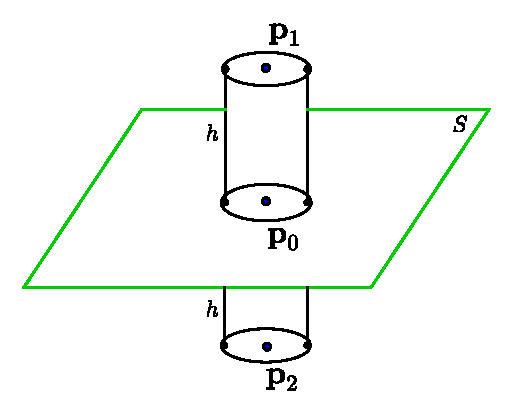
\includegraphics[scale=1]{interface_elastici}
\caption{\textit{Cilindro de dimens\~oes infinitesimais dividido pela interface separadora dos meios 1 e 2.}}
\label{fig.interface_elastici}
\end{figure}
Considerando ainda que cada um dos pontos $\mathbf{p}_1$ e $\mathbf{p}_2$ s\~ao os centros de cada uma das bases do cilindro, temos que os pontos $\mathbf{p}_0$, $\mathbf{p}_1$ e $\mathbf{p}_2$ est\~ao alinhados. Utilizando novamente a equa\c{c}\~ao \ref{eq.forca_total_3} e desprezando as for\c{c}as aplicadas na parede do cilindro (j\'a que vamos fazer $h\to 0$), temos que o equil\'ibrio de for\c{c}as aplicadas ao cilindro \'e dado por 
\begin{equation*}
\mathbf{F}=\mathbf{F}(\mathbf{p}_1)+\mathbf{F}(\mathbf{p}_2)+f
\end{equation*} 
onde $f$ \'e uma for\c{c}a de campo. Utilizando a segunda lei de Newton, utilizando a equa\c{c}\~ao \ref{eq.tensao_media} e desprezando as for\c{c}as de campo, temos
\begin{equation*}
\rho\,dh\,dA\frac{d\mathbf{v}}{dt}=\mathbf{T}(\mathbf{p}_1,\mathbf{n})dA+\mathbf{T}(\mathbf{p}_2,-\mathbf{n})dA.
\end{equation*} 
Fazendo o limite quando $h\to 0$ e mantendo constantes as \'areas das bases do cilindro, temos que os pontos $\mathbf{p}_i$ convergem para $\mathbf{p}_0$, e a equa\c{c}\~ao acima se torna
\begin{equation*}
\mathbf{T}(\mathbf{p}_0,\mathbf{n})-\mathbf{T}(\mathbf{p}_0,\mathbf{n})=\mathbf{0}.
\end{equation*}
Como o ponto $\mathbf{p}_0$ \'e tomado arbitrariamente, temos que o salto do tensor de tens\~oes ao longo da superf\'icie $S$ \'e nulo
\begin{equation*}
\left[\left[\mathbf{T}\right]\right]=\mathbf{0}.
\end{equation*}
Considerando um modelo onde uma camada n\~ao vai invadir a outra temos que a componente normal do vetor de deslocamento $\mathbf{u}\in S$ \'e nula. Da mesma forma, considerando que uma camada n\~ao desliza sobre a outra, temos que as componentes tangenciais de $\mathbf{u}$ tamb\'em s\~ao zero, e da\'i assumimos que o salto de $\mathbf{u}$ \'e nulo bem como sua velocidade,
\begin{equation*}
\left[\left[\mathbf{u}\right]\right]=\mathbf{0}\quad\text{e}\quad\left[\left[\frac{\partial}{\partial t}\mathbf{u}\right]\right]=\mathbf{0}.
\end{equation*}

